\documentclass{IEEE_lsens}
\usepackage{textcomp}
\usepackage{cite}
\ifCLASSINFOpdf
  \usepackage[pdftex]{graphicx}
\else
\fi
\usepackage[T1]{fontenc} 
\usepackage{amsmath}
\interdisplaylinepenalty=2500
\usepackage[cmintegrals]{newtxmath}
\usepackage{bm}
\usepackage{array}
\usepackage{float}
\usepackage[caption=false,font=footnotesize,labelfont=sf,textfont=sf]{subfig}
\usepackage{url}
\newcommand\MYhyperrefoptions{hypertexnames=true, bookmarks=true,
bookmarksnumbered=true, pdfpagemode={UseOutlines}, plainpages=false,
pdfpagelabels=true, colorlinks=true, linkcolor={black},
citecolor={black}, urlcolor={black}}
\ifCLASSINFOpdf
\else
\fi
\providecommand{\hypersetup}[1]{\relax}
\providecommand{\texorpdfstring}[2]{#1}
\hypersetup{pdftitle={Bare Demo of IEEE\_lsens.cls for IEEE Sensors Letters},%<!CHANGE!
pdfsubject={Typesetting},%<!CHANGE!
pdfauthor={Michael D. Shell},%<!CHANGE!
pdfkeywords={Class, IEEE, IEEE\_lsens, IEEE Sensors Letters, LaTeX, Typesetting, TeX}}%<^!CHANGE!}
\hyphenation{op-tical net-works semi-conduc-tor}
\begin{document}
\markboth{Vol.~X, No.~X, Feb~2026}{0000000}
\IEEELSENSarticlesubject{Sensor Systems}
\title{Physics-Informed Incremental Domain Adaptation Network for Gas Sensor Drift Compensation}
\author{\IEEEauthorblockN{~Pritam~Khan\IEEEauthorieeemembermark{1},~Shashank~Acharya~and~Bhumi~Awasthi}
\IEEEauthorblockA{Department of Computational Intelligence, SRM Institute of Science and Technology, Kattankulathur 603203, India \\ \IEEEauthorieeemembermark{1}Member, IEEE
}%
\thanks{This work acknowledges the support rendered by the Centre for Computational Sustainability, SRM Institute of Science and Technology, Kattankulathur, India.\\Corresponding author: Pritam Khan (e-mail: pritamk249@gmail.com).}
%\thanks{Associate Editor: xx}%
\thanks{Digital Object Identifier: 10.xx}}
\IEEELSENSmanuscriptreceived{Manuscript received February 10, 2026}%; revised September 26, 2024; accepted October 10, 2024.}% Date of publication  , 2024; date of current version xx, 2024.}
\IEEEtitleabstractindextext{%
\begin{abstract}
Gas sensor arrays suffer from long-term drift, which progressively distorts their baselines and sensitivities and causes models trained on early data to fail on later measurements. This work proposes a PI-IDAN (Physics-Informed Incremental Domain Adaptation Network) that explicitly models gas sensors' response with a physics head while incrementally aligning representations across drifted batches without requiring new labels. The framework consists of a Siamese encoder with three heads: a gas classifier, a physics projection head that enforces the Yamazoe logarithmic power law and monotonic baseline drift, and a drift discriminator with gradient reversal for representation alignment. Lastly, a two‑phase training scheme with supervised initialization on early labeled batches is followed by pseudo‑label‑driven, class‑balanced memory replay and domain‑adaptation alignment on later unlabeled batches. Together, these design choices yield a method that is both physically grounded and resilient to high drifts on the UCI gas sensor array drift dataset. PI‑IDAN achieves an average accuracy of about 82.5\%, improving over standard IDAN and other deep‑learning baselines such as 1D CNNs and LSTMs in long‑drift settings. This demonstrates embedding sensor physics into incremental domain‑adaptation learning substantially advances the state-of-the-art in drift compensation for gas sensor array systems.
\end{abstract}

\begin{IEEEkeywords}
Gas sensor drift compensation, Physics-informed learning, Gas sensors, Incremental domain adaptation, Catastrophic forgetting.
\end{IEEEkeywords}}

% If you want to put a publisher's ID mark on the page, you can do it like
% this:
%\IEEEpubid{1949-307X \copyright\ 2017 IEEE. Personal use is permitted, but republication/redistribution requires IEEE permission.\\
%\url{http://www.ieee.org/publications\_standards/publications/rights/index.html} for more information.}
% Remember, if you use this, you must call \IEEEpubidadjcol in the second
% column for its text to clear the IEEEpubid mark.
% make the title area
\maketitle
\section{Introduction}
Gas sensor array systems are widely used in environmental monitoring, industrial safety, smart cities, and air quality surveillance due to their low cost, compactness, and high sensitivity to various gases \cite{dutta2023road}. In these applications, arrays of partially selective sensors are used to classify gas types and estimate concentration over long periods, often months or years \cite{vergara2012chemical}. However, the long‑term reliability of such systems is fundamentally constrained by sensor drift: gradual changes in baseline and sensitivity caused by aging, poisoning, environmental fluctuations, and fabrication variability \cite{dennler2022drift}. Studies on the canonical gas sensor array drift (GSAD) dataset has shown that models trained on early batches can suffer severe accuracy degradation on later batches, even when the target gases and operating protocol remain nominally unchanged, which is unacceptable in safety‑critical monitoring and regulatory compliance scenarios \cite{vergara2012chemical,dennler2022drift}.

Drift presents a unique challenge for sensors due to its non-linear nature, dependence on slow processes, and susceptibility to noise and environmental variations. Conventional approaches, such as periodic or static recalibration, do not sufficiently address the impact of drift \cite{dennler2022drift}. The most successful methods developed today blend the use of machine learning with sensor-level signal corrections. For instance, ensemble-based classifiers that utilize GSAD data outperform individual classifiers because they consider multiple decision boundaries. In addition to ensemble and average models, LSTM-SVM (Long Short-Term Memory-Support Vector Machine) hybrid classifiers utilize the time evolution of the sensor response more effectively, allowing for more accurate tracking of changes in the sensor response over time \cite{vergara2012chemical, zhao2019sensor}. 

Traditional supervised models (SVM, Incremental SVM), convolutional and recurrent neural networks (1D‑CNN, TimesNet, LSTM), and even domain‑adversarial approaches such as standard IDAN represent the current state-of-the-art for learning‑based drift compensation \cite{dong2025real, zhao2019sensor}, yet these methods share three critical limitations: they generally require labeled data whenever drift conditions change, they treat drift as a generic statistical shift without following physical laws, and they lack strong continual learning mechanisms to prevent catastrophic forgetting across long sequences of drifted conditions \cite{dennler2022drift}. Recent work also highlights random forests as strong, robust learners for noisy tabular data and useful baselines for classification and error handling under drift \cite{salman2024random}, however, such studies focus on generic robustness and do not incorporate sensor-specific physics or explicit mechanisms for incremental domain adaptation over long time horizons. These shortcomings of existing approaches are particularly critical in realistic deployments, with the most severe drift often occurring in the later stages of operation, where the class distributions are generally imbalanced \cite{dennler2022drift}. Moreover, semi‑supervised and unsupervised approaches often rely on heuristics developed for specific sensor types and are sensitive to changes in drift patterns or class distributions, while sequential deep‑learning pipelines can degrade on earlier conditions after training on new batches \cite{vergara2012chemical, zhao2019sensor}.
 
 To address these limitations, this letter introduces a novel Physics‑Informed Incremental Domain Adaptation Network (PI‑IDAN) for long‑term drift compensation in gas sensor array systems. PI‑IDAN incorporates a novel physics head that enforces a Yamazoe logarithmic relationship between concentration and response. It also constrains baseline evolution to be monotonic and class‑consistent across batches, ensuring that the learned behavior remains physically realistic even as drift accumulates \cite{hua2018theoretical}. On top of this physics‑informed backbone, PI‑IDAN uses a convolutional encoder, gas classifier, and drift discriminator trained in two phases: a supervised initialization on early labeled batches, followed by memory‑replay‑based incremental adaptation with pseudo‑labels, domain‑adversarial alignment, and physics‑guided losses across unlabeled, drifted batches \cite{lee2024incremental, zhang2025lithium}. Empirical results on a long‑term drift benchmark show that this design not only improves overall accuracy over standard IDAN and strong deep learning baselines, but also maintains significantly higher performance in mid‑to‑late drift, where traditional %and domain‑adversarial 
 models degrade, providing concrete evidence that explicitly embedding sensor physics into incremental domain adaptation effectively fixes key failure modes of existing models \cite{dennler2022drift}.
\section{Gas classification with sensor drift compensation using PI-IDAN}
In this work, a Physics-informed Incremental Domain Adaptation approach for sensor drift compensation and gas prediction is presented. We have a labeled source domain $D_S = \{(\textit{\textbf{x}}_i^s, y_i^s)\}_{i=1}^{N_s}$, where $\textit{\textbf{x}}_\text{i}^\text{s}$ denotes the $i$-th feature vector in the source domain, $y_i^s$ represents its corresponding gas class label, and $N_s$ is the total number of labeled source samples.Also, we have an unlabeled target domain $D_{T_1}, D_{T_2}, \dots, D_{T_J}$, where $D_{T_j}$ represents the $j$th sequential target batch, with $J$ being the total number of target domains. We aim to build a model $f_0$ that is able to classify gases correctly while adapting sequentially to each new domain $D_{T_j}$ and differentiating between drift and sensor signals using an incremental domain adaptation technique paired with physics-informed knowledge for robust and scientifically grounded predictions.
To ensure that there is no chance of data leakage between batches, we compute the Z-score statistics (mean, standard deviation) only for the first batch and keep these values fixed while processing the rest of the batches. This allows the model to experience drift exactly as it would in a practical deployment and maintain the ``aging'' pattern within the dataset \cite{dennler2022drift}.
\subsection{Proposed Framework of Physics-Informed Incremental Domain Adaptation for Sensor Drift Compensation}
 \begin{figure}[H]
  \centering
 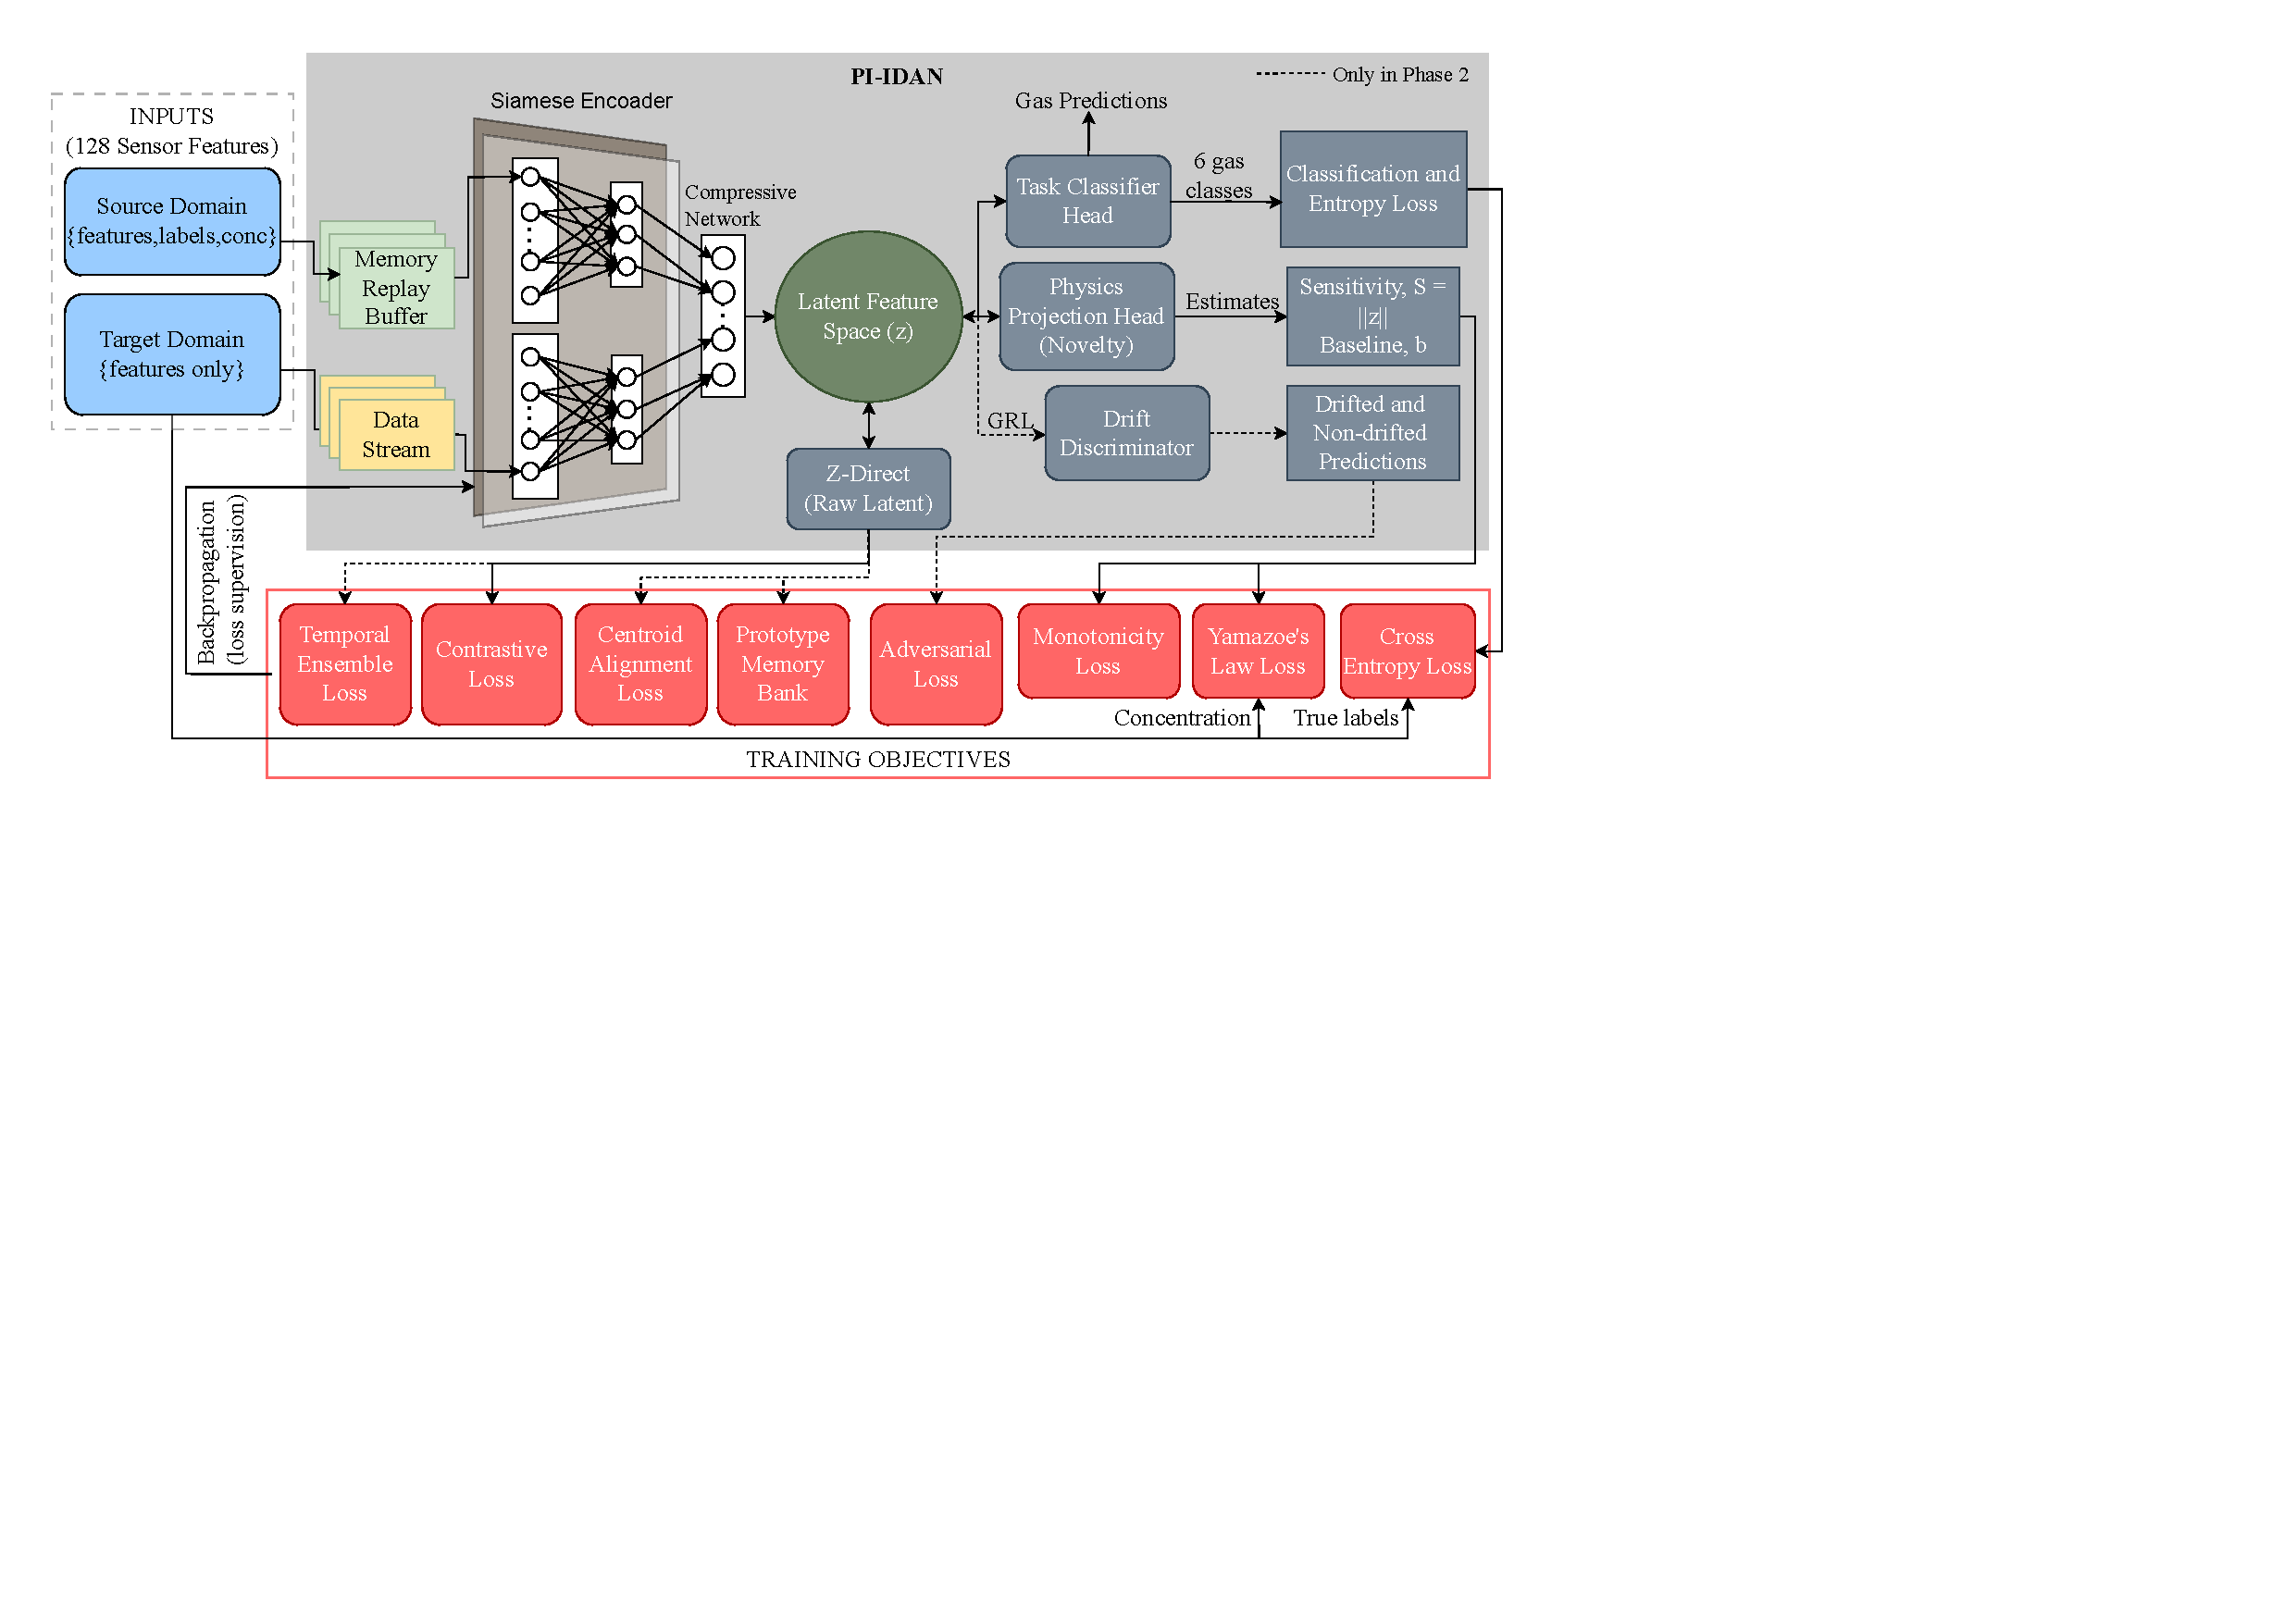
\includegraphics[width=1.0\columnwidth, trim=0cm 15.4cm 13.5cm 0cm, clip]{images/Archie.drawio.pdf}
 \caption{The proposed PI-IDAN architecture diagram.}
 \label{fig:my_architecture}
 \end{figure}
The PI-IDAN aids in the compensation of sensor drift by using two training phases. As shown in Fig.\ref{fig:my_architecture}, the proposed architecture contains a common Siamese architecture encoder that generates a 64-dimensional latent feature vector representation of a 128-dimensional sensor response and branches into three unique heads. They are a Task Classifier for identifying gases, a Physics Projection Head that imposes physical constraints, and a drift Discriminator for adaptation alignment\cite{dong2025real, zhang2025lithium}. There are two phases to the training process: Phase 1 source domain is used to create a baseline source model using labeled data. In contrast, the Phase 2 target domain gradually adapts the model using physics-constrained domain adaptation to accommodate incremental additions of unlabeled target batches \cite{lee2024incremental}.
\subsubsection*{Phase 1: Source Domain Training}
In the first stage, the model will learn to extract relevant characteristics of a dataset with labeled source domain samples while simultaneously establishing representations that satisfy the physical principles. The source domain is passed through a Siamese Encoder for feature extraction and compression. The input is transformed to 1-D vector and passed through three convolutional blocks \cite{ige2024state}.
The first layer employs a kernel of size $k=9$ with striding $s=8$ and padding $p$ = 4 to capture long-term dependencies of the sensor's signal. Batch normalization, ReLU activation, and dropout (0.1) are implemented after each layer for stable training. The second layer utilizes a dilation $d=4$ and kernel $k=3$. The dilation increases the receptive field to 17 samples without increasing parameters. The third layer, with a kernel size of 3 and stride of 1, extracts features from the input.
The resulting 2048-dimensional tensor passes through a fully connected three-layer compressive network  ($2048 \rightarrow 512 \rightarrow 128 \rightarrow 64$) with ReLU activations and dropout $p=0.2$, producing the 64-dimensional latent vector $\textbf{z}$.
The latent vector $\textbf{z}$ is passed to the task classifier, which employs a two-layer Neural Network ($64 \rightarrow 32 \rightarrow 6$) with ReLU activation and dropout $p=0.1$ in the hidden layer. The classifier predicts gas category probabilities, optimized using cross-entropy loss. At the same time, we introduced a z-direct step, which applies supervised contrastive learning directly on the latent vector $\textbf{z}$ to obtain a geometry‑refined representation, where samples of the same gas are pulled together, and samples of different gases are pushed apart \cite{khosla2020supervised}.
%This will minimize contrastive loss $\mathcal{L}_{\text{cont}}^1 = -\frac{1}{N}\sum_{i=1}^{N} \frac{1}{|P(i)|} \sum_{p \in P(i)} \log \frac{\exp(\text{sim}(z_i, z_p)/\tau)}{\sum_{a \neq i} \exp(\text{sim}(z_i, z_a)/\tau)}
%where\text{``sim''}$ denotes cosine similarity and $ \tau = 0.07$ is the temperature.
Similarly, the same latent vector $\textbf{z}$ is passed through the physics head, which is implemented using a two-layer Multi-Layer-Perceptron ($64 \rightarrow 32 \rightarrow 2$) with ReLU activation. The physics head is trained to predict 2 quantities that ensure the descriptions remain true to the physical laws describing the gas sensor’s behavior. The first prediction is the Sensitivity Magnitude, $S$, obtained by the Yamazoe Power Law, which explains that the sensitivity magnitude is related to the logarithmic gas concentration\cite{hua2018theoretical}, and this law is enforced by power loss $\mathcal{L}_\text{power1}$ defined by the Mean Squared Error (MSE) between the predicted sensitivity magnitude and the target value derived from the ground-truth concentration.
$
 \mathcal{L}_{\text{power1}} = \text{MSE}(S, w \cdot \log(C) + b)
$
Where $C$ is the known gas concentration from source labels, and $w$ (initialized to 0.5), $b$ (initialized to 0.0) are learnable parameters encoding the power law relationship between concentration and sensitivity. The second prediction is the Baseline Estimate $b$, which is the sensor's resistance in the absence of any gas. The estimate $b$ is used to calculate the monotonicity loss $\mathcal{L}_\text{mono1}$ which penalizes the deviation from the expected drift direction and ensures that the drift is unidirectional.
$
\mathcal{L}_{\text{mono1}} = \text{ReLU}(-\Delta b \cdot \text{dir})
$
 where $\Delta b = b_j - b_{j-1}$ represents the change between the current mean baseline estimate and the previous batch's baseline. The term $\text{dir} \in \{+1, -1\}$ encodes the expected drift direction determined from the initial source batches\cite{vergara2012chemical}.
The task, contrastive, and physics component losses combine to calculate total loss $\mathcal{L}_{\text{Phase1}}$ as:
\begin{equation}
 \mathcal{L}_{\text{Phase1}} = \mathcal{L}_{\text{task1}} + \lambda_{\text{cont1}} \mathcal{L}_{\text{cont1}} + \lambda_{\text{power1}} \mathcal{L}_{\text{power1}} + \lambda_{\text{mono1}} \mathcal{L}_{\text{mono1}}
\end{equation}
while training the model. Here $\lambda_{\text{cont1}} = 1.0$, $\lambda_{\text{power1}} = 0.1$, and $\lambda_{\text{mono1}} = 0.1$ are the penalty hyperparameters corresponding to each loss. Training proceeds for 20 epochs using the Adam optimizer with a learning rate $\eta = 0.001$. The baseline estimate from this phase, $b_0$, is stored as the physics reference for subsequent adaptation.
For the Mean Teacher configuration, the Exponential Moving Average (EMA) `teacher' model is initialized with a copy of the `student' model. The parameters of the student's encoder and classifier, $\theta$, are tracked by the parameters of the teacher model's EMA, $\theta_{\text{EMA}}$, with a momentum coefficient $\alpha = 0.999$. The teacher model is then updated after every batch according to the rule $\theta_{\text{EMA}} \leftarrow \alpha \cdot \theta_{\text{EMA}} + (1 - \alpha) \cdot \theta$.

\subsubsection*{Phase 2: Incremental Physics-Constrained Adaptation}
During Phase 2, the model adapts sequentially to each new target domain batch $D_{T_j}$ with temporal drift.
%Before adapting to each new batch , the output layer of the domain discriminator is increased in size by adding one neuron to the prior batch.
%he existing weights of the domain discriminator are kept unchanged, and the new weights are initialized randomly using a Gaussian distribution ($\sigma = 0.01$).
The drift discriminator is used to discriminate between the drifted and non-drifted batches.
%This allows the domain discriminator to facilitate multi-class classification across all the existing batches. 
During adaptation, each labeled sample $(\textit{\textbf{x}}_i^s, y_i^s)$ for each $i$-th feature vector corresponding to the source domain from a memory replay buffer containing previous batches (source batch) and unlabeled samples $\textit{\textbf{x}}_j^t$ from the current target batch $D_{T_j}$ are processed in parallel and passed through the encoder to produce latent vectors $\textbf{z}_\text{s}$ and $\textbf{z}_\text{t}$ respectively.
The latent vectors are passed through a Gradient Reversal Layer (GRL) to the drift  Discriminator. %GRL reverses the gradient during backpropagation. 
The discriminator consists of a hidden layer ($64 \rightarrow 32$) with ReLU and dropout ($p=0.1$), followed by the output layer. Next, the adversarial loss is obtained as $\mathcal{L}_{\text{adv}} = \text{CE}(D(\textbf{z}_s), d_s) + \text{CE}(D(\textbf{z}_t), d_t)$, where CE is binary cross-entropy, $D(\textbf{z}_s)$ and $D(\textbf{z}_t)$ are the drifted and non-drifted predicted batches by the discriminator for $\textbf{z}_s$ and $\textbf{z}_t$ respectively, $d_s$ and $d_t$ are the source batch and the currently drifted batch respectively. %This adversarial loss encourages domain-invariant features for all target samples \cite{zhang2025lithium}.
The source latent vector $\textbf{z}_\text{s}$ is passed through the task classifier to compute supervised task loss $\mathcal{L}_{\text{task2}}$, which prevents catastrophic forgetting through continuous replay of labeled source samples\cite{lee2024incremental}. The classifier learning rate $\eta_\text{cls}$ is 10 times lower than the encoder to preserve source knowledge while allowing gradual adaptation.
%For unlabeled target samples, we create a cloned copy of the current model and use it to generate pseudo-labels $\hat{y}_t$ from its predicted class probabilities. To avoid noisy supervision, we retain only high-confidence pseudo-labels: for each class, only samples whose confidence exceeds the class-wise median, with a minimum threshold of 0.4, are kept. These high-confidence target samples are then combined with labeled source samples,
%$\mathbf{z}_{\text{combined}} = [\mathbf{z}_s; \mathbf{z}_t^{\text{high-conf}}]$, 
%$y_{\text{combined}} = [y_s; \hat{y}_t^{\text{high-conf}}]$,
%for joint contrastive learning (pulling same-class features together), cross-domain centroid alignment
%$\mathcal{L}_{\text{cross}} = \sum_{c=1}^{6} \text{MSE}(\bar{\mathbf{z}}_s^{(c)}, \bar{\mathbf{z}}_t^{(c)})$,
% 5and prototype-based classification
%$\mathcal{L}_{\text{proto}} = \text{CE}\!\left(\frac{\mathbf{z}_s \cdot P^{T}}{\tau}, y_s\right)$
%with temperature $\tau = 0.1$.
A pseudo-label is created using the Mean Teacher Algorithm by taking the Exponential Moving Average (EMA) of the encoder and classifier \cite{tarvainen2017mean}. The pseudo-label $\hat{y}^t_j$ for a given unlabeled target sample $\textit{\textbf{x}}^t_j$ is computed by $\hat{y}^t_j = \arg\max \text{softmax}(f_{\text{EMA}}(E_{\text{EMA}}(\textit{\textbf{x}}^t_j)))$ where $\textit{\textbf{x}}^t_j$ represents the raw sensor input from the current drifted batch. The terms $E_{\text{EMA}}$ and $f_{\text{EMA}}$ denote the Teacher encoder and Teacher classifier respectively. These components process the raw input to produce a stable prediction, independent of the student network's current fluctuations. The temporal ensemble loss $\mathcal{L}_{\text{te}}$ is computed as the MSE between the student and the teacher networks by penalizing the deviation from the EMA.
%A method for filtering reliable pseudo-labels is based on the confidence of each sample.
For reliable pseudo-label filtering, only sample pairs with confidence above each class median (minimum 0.4) are included during training. The high-confidence target samples along with their pseudo-labels are appended to the source samples that yields the combined latent vector $\textbf{z}_{\text{combined}} = [\textbf{z}_s; \textbf{z}_t^{\text{high-conf}}]$ with combined labels $y_{\text{combined}} = [y^s_i; \hat{y}_j^{t_\text{high-conf}}]$
where $\textbf{z}_t^{\text{high-conf}}$ is the selected target latent vector with  $\hat{y}_j^{t_\text{high-conf}}$ being the generated pseudo-labels.
%$z_{\text{combined}}$ is aligned with three losses.
$\textbf{z}_{\text{combined}}$ is optimized using three alignment objectives;
first, supervised contrastive learning \cite{khosla2020supervised}, which groups the same-class samples across multiple domains. Second, cross-domain centroid alignment $\mathcal{L}_{\text{cross}}$ is used to synchronize the centroid of the source and target domains. Lastly, the prototype-guided adaptation strategy $\mathcal{L}_{\text{proto}}$ updates a global memory bank to maintain a steady gas representation \cite{du2023prototype}.
Simultaneously, to ensure physical consistency, the target vectors $\textbf{z}_t$ pass through the physics head to estimate the baseline $b_j$ and calculate the monotonicity loss to enforce unidirectional baseline drift. This prevents physically impossible random fluctuations during adaptation.
% the joint contrastive learning pulls the same classes together, the alignment of the centroids across domains to align the distribution of the class, $\mathcal{L}_{\text{cross}} = \sum_{c=1}^{6} \text{MSE}(\bar{z}_s^{(c)}, \bar{z}_t^{(c)})
% $ and the prototype memory bank to update the centroids $
% \mathcal{L}_{\text{proto}} = \text{CE}\left(\frac{z_s \cdot P^T}{\tau}, y_s\right),$where $\tau$= 0.1
%The total incremental adaptation loss combines all components in phase 2.
Combining all the objectives of phase 2, the total incremental adaptation loss is obtained as:
\begin{equation}
\begin{split}
\mathcal{L}_{\text{Phase2}} = & \,
\lambda_{\text{task2}} \mathcal{L}_{\text{task2}} + \lambda_{\text{adv}} \mathcal{L}_{\text{adv}} + \lambda_{\text{cont2}} \mathcal{L}_{\text{cont2}} + \lambda_{\text{mono2}} \mathcal{L}_{\text{mono2}} \\
& + \lambda_{\text{cross}} \mathcal{L}_{\text{cross}} + \lambda_{\text{proto}} \mathcal{L}_{\text{proto}} + \lambda_{\text{te}} \mathcal{L}_{\text{te}}
\end{split}
\end{equation}
In our experiments, these hyperparameters are empirically set to
$\lambda_{\text{task2}} = 0.5$, $\lambda_{\text{adv}} = 0.1$,
$\lambda_{\text{cont2}} = 1.5$, $\lambda_{\text{mono2}} = 0.5$,
$\lambda_{\text{cross}} = 0.3$, $\lambda_{\text{proto}} = 0.5$, and
$\lambda_{\text{te}} = 0.5$.
Adaptation proceeds using the Adam optimizer with a learning rate $\eta = 0.0001$ (10 times lower than Phase 1), Gradient clipping (max norm 1.0) prevents instability. After each batch, $b_j$ is recorded for the next iteration's monotonicity constraint, and the EMA model is updated accordingly.

\section{RESULTS AND DISCUSSION}
The proposed PI-IDAN model uses the UCI Gas Sensor Array Drift Dataset (GSAD)\cite{vergara2012chemical}, that represents a realistic deployment scenario spanning over the course of 36 months. The data consists of 10 sequentially collected batches from an array of 16 metal oxide gas sensors that provide a total of 128 dimensions of features representing 6 different classes of gases, along with their corresponding concentration levels at an isothermal condition.

\subsection{Performance Evaluation of the PI-IDAN Framework}

% \begin{table}[h!]
% \centering
% \caption{Performance Comparison: PI-IDAN vs. Non-Physics Baseline}
% \label{tab:comparison_summary}
% \begin{tabular}{lccc}
% \hline
% \textbf{Metric}    & \textbf{PI-IDAN} & \textbf{Non-Physics} & \textbf{Improvement} \\ \hline
% Accuracy & 82.54\%  & 76.29\%  & +6.29\% \\
% Precision & 80.22\% & 74.98\% & +5.24\% \\
% Recall & 77.31\% & 72.46\% & +4.85\% \\
% F1-Score & 75.19\% & 67.78\% & +7.41\%\\ \hline
% \end{tabular}
% \end{table}

\begin{figure}[]
 \centering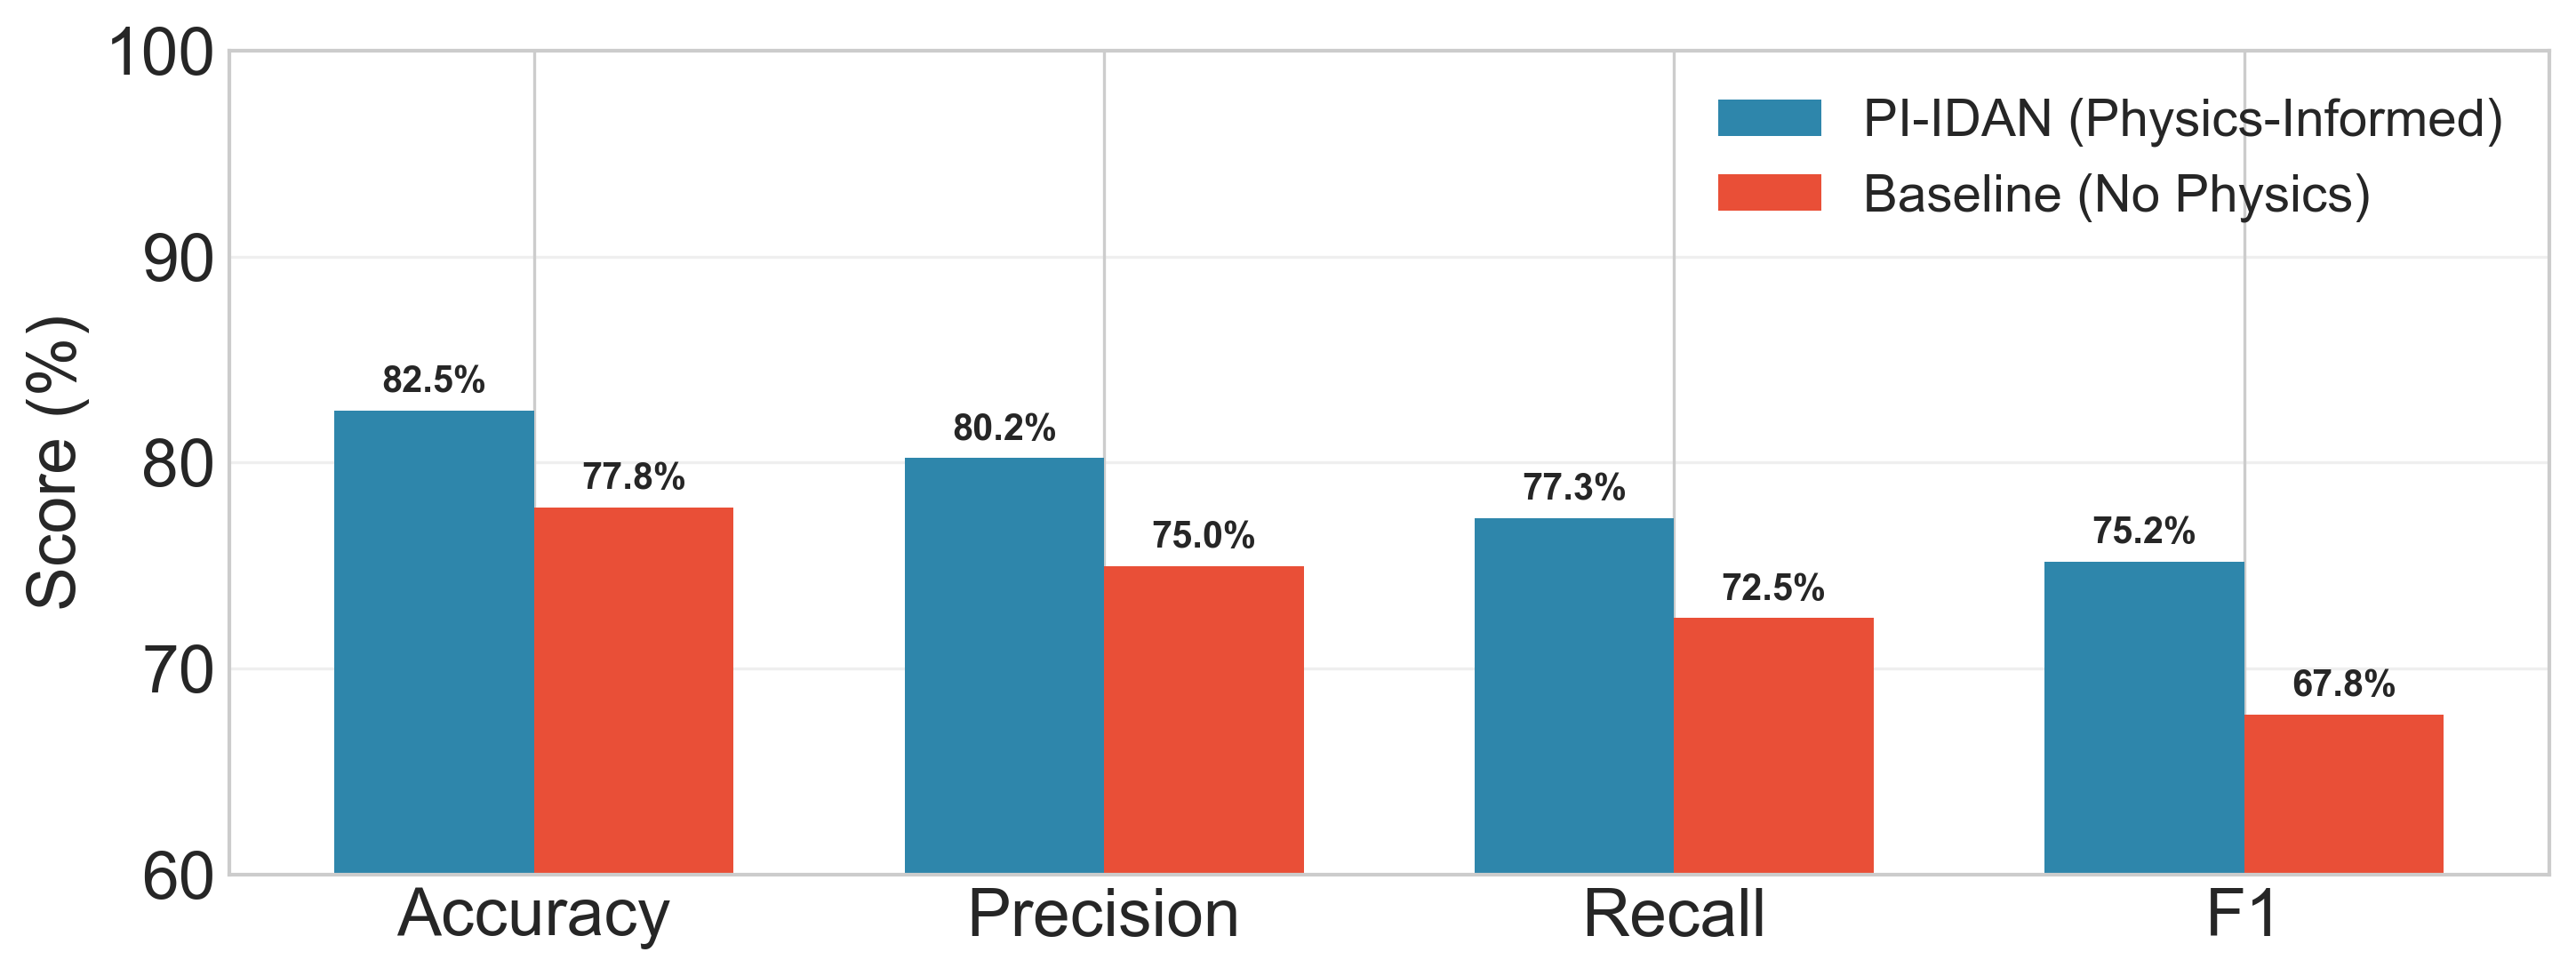
\includegraphics[width=0.75 \columnwidth]{images/summary_comparison2.png}
 \caption{Average performance comparison of PI-IDAN and baseline models across all branches}
 \label{fig:imp_over_batches}
\end{figure}

The non-physics model tends to overfit the sensor data as it learns through its drift and degradation, whereas the physical laws prevent physics-informed data from overfitting. Figure~\ref{fig:imp_over_batches} shows an average improvement of 4.7\% for the PI-IDAN model over the baseline (non-physics) model. Analysis of per-batch results reveals that the physics-informed advantage is most significant in later batches, where the drift is more severe. The consistent improvement in the performance metrics ensures that the physics-informed models not only provide better accuracy but also stable and physically grounded meaningful effects, as can be observed from the sensor drift compensation.

%Figure~\ref{fig: graph} represents a two-dimensional t-SNE visualization of the learned multi-dimensional latent feature space. As shown in Figure~\ref{fig:3a}, the PI-IDAN framework clusters the samples of the same gas into small and well-separated groups. It shows that the latent features are highly discriminative and can handle drift easily. Figure~\ref{fig:3b} shows that there is a great overlap among various batches of each gas cluster, thereby highlighting good inter-batch alignment.
%The results of Figure ~\ref{fig: graph} establish that PI-IDAN acquires drift-invariant representations with strong class separability to effectively handle drift

The results in Figure~\ref{fig: graph} establish that PI-IDAN acquires class-separable and drift-invariant representations for handling drift. This work is being done by t‑SNE (t-distributed Stochastic Neighbor Embedding) that projects the high‑dimensional latent features learned into two dimensions. This ensures that points closer on the plot have similar latent representations, while distant points are dissimilar, as observed from Figure~\ref{fig:3a}. Figure~\ref{fig:3b} demonstrates that there is a great overlap among various batches of each gas cluster, thereby highlighting good inter-batch alignment.

\begin{figure}
\centering
\subfloat[Latent space by gas class]{
  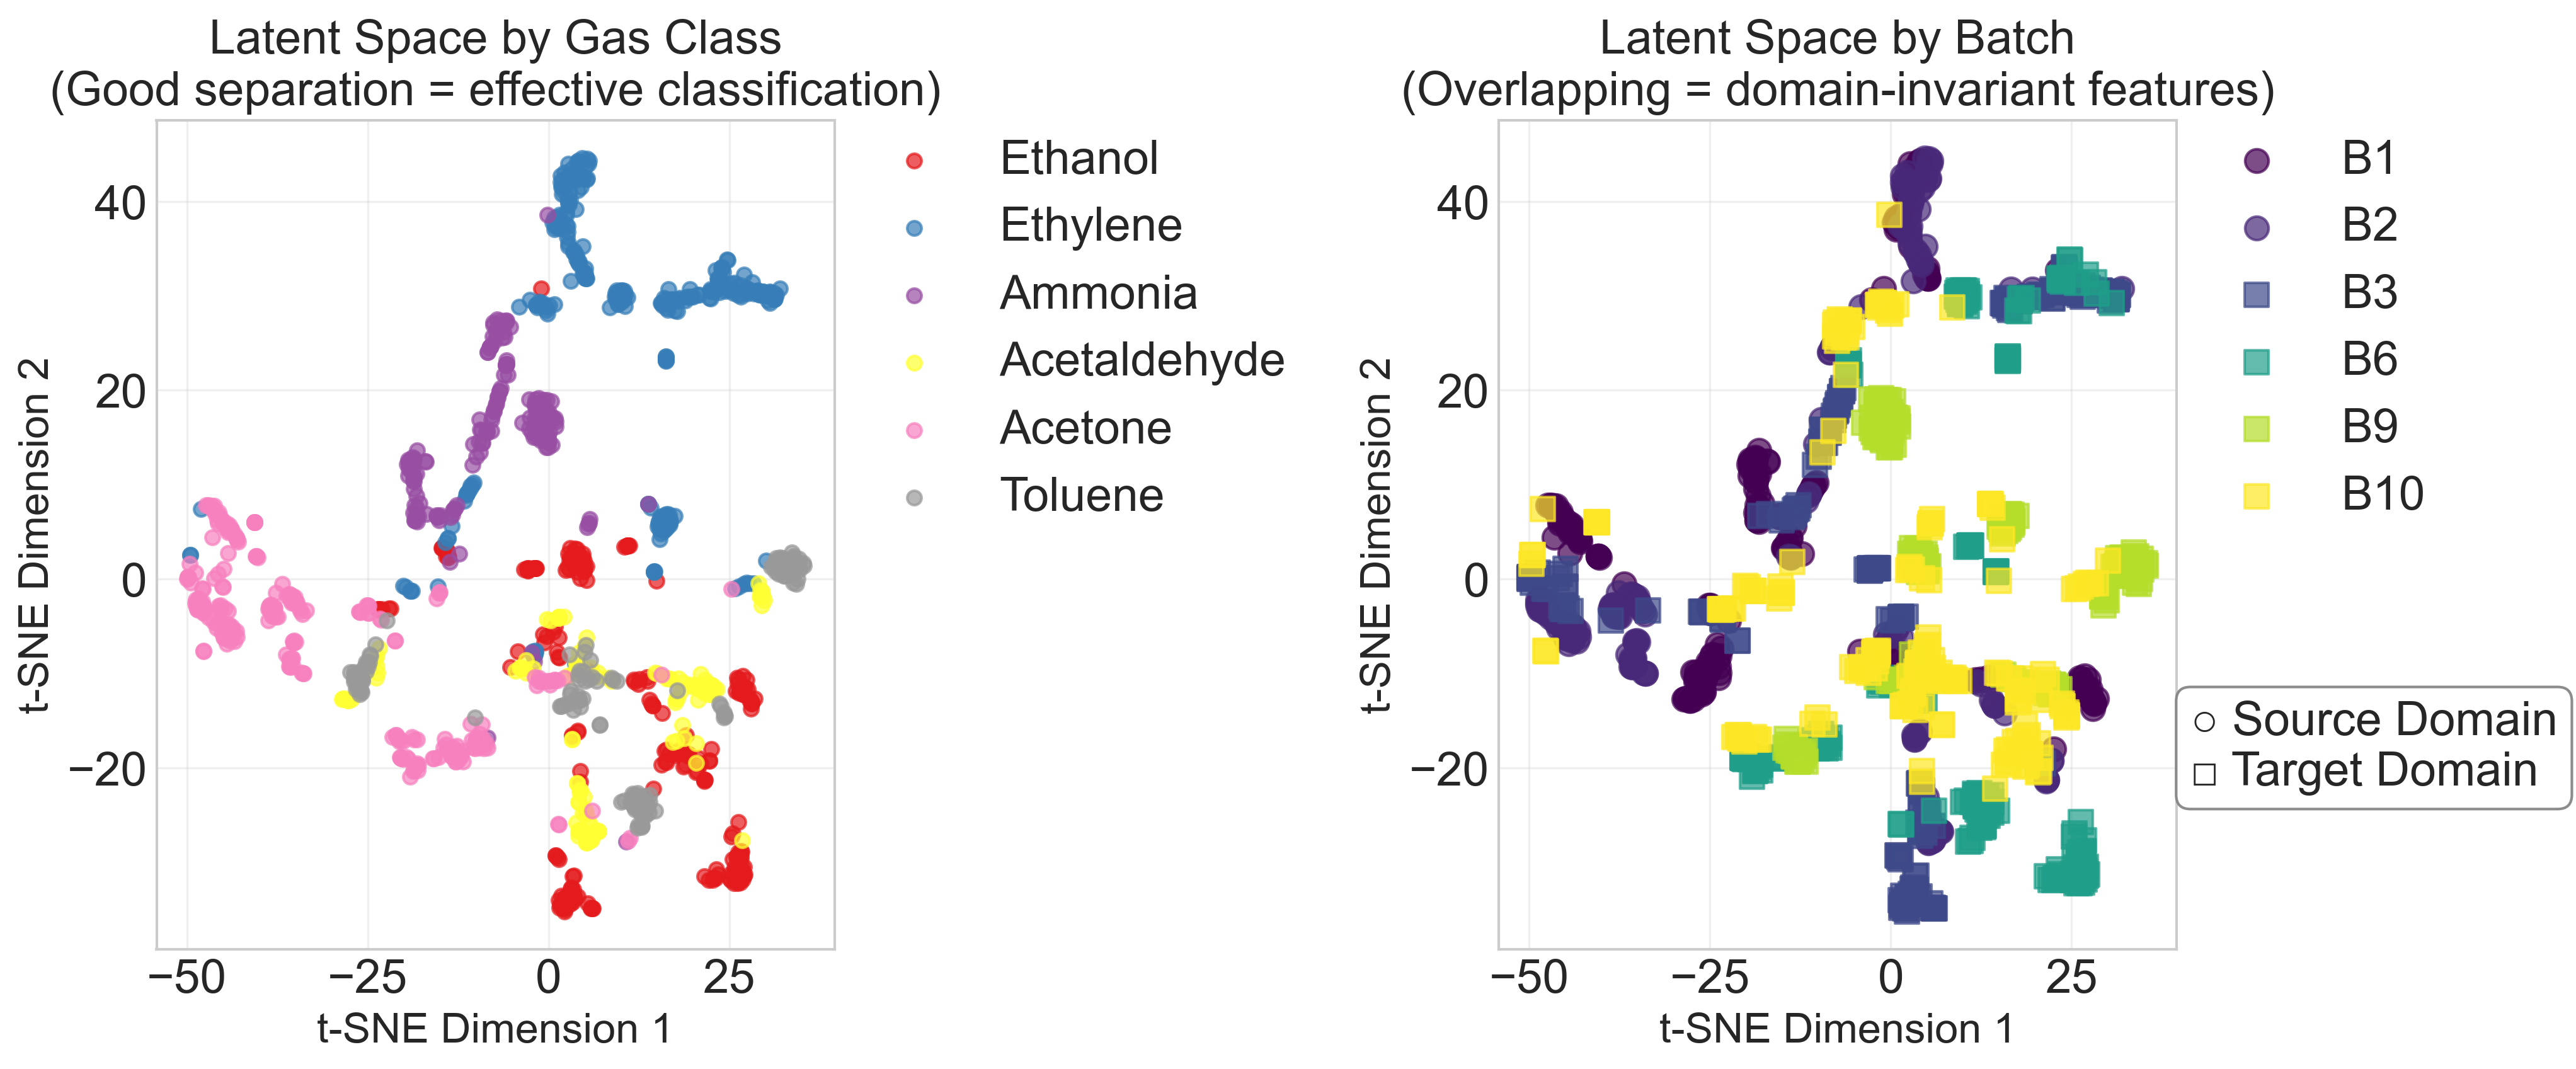
\includegraphics[
    width=0.48\linewidth,trim=0 0 490 0,clip
  ]{images/tsne_latent_space.png}
  \label{fig:3a}
}
\hfill
\subfloat[Latent space by batch]{
  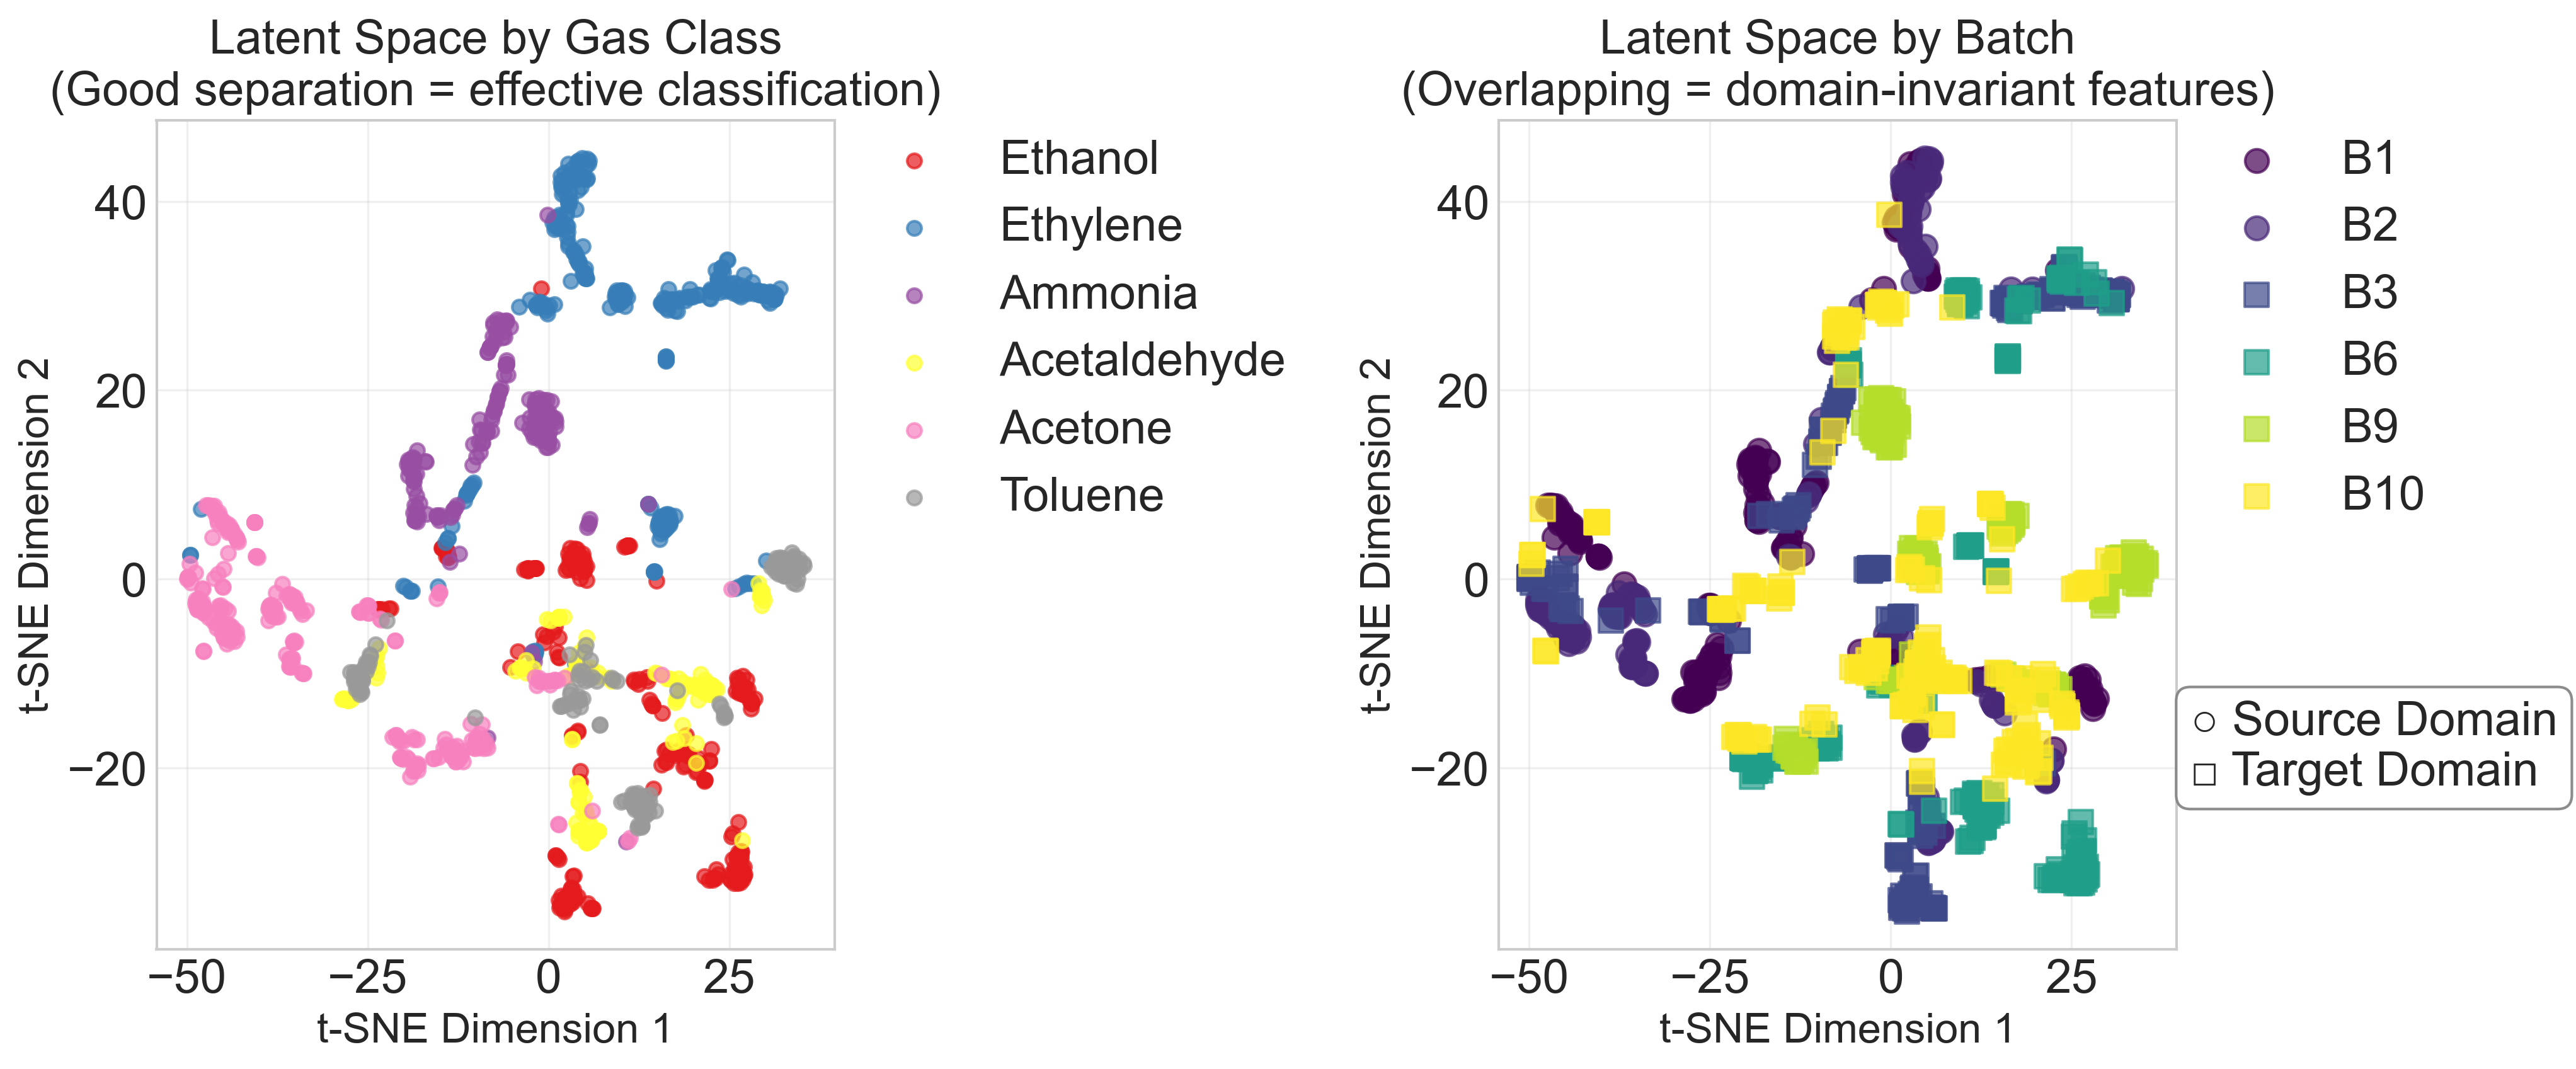
\includegraphics[
    width=0.48\linewidth,trim=490 0 0 0,clip
  ]{images/tsne_latent_space.png}
  \label{fig:3b}
}

\caption{t-SNE Embedding of PI-IDAN Latent Representations: Class-Wise Separation and Cross-Domain Alignment.}
\label{fig: graph}
\end{figure}

\begin{table}[h]
\centering
\caption{Detailed Performance Metrics by Batch with Variability (Phase 2 Adaptation)}
\label{tab:performance_metrics_pm}
\resizebox{\columnwidth}{!}{
\begin{tabular}{lcccc}
\hline
\textbf{Batch ID} 
& \textbf{Accuracy (\%)} 
& \textbf{Precision (\%)} 
& \textbf{Recall (\%)} 
& \textbf{F1-Score (\%)} \\ \hline

Batch 3  
& $99.2 \pm 0.6$ 
& $82.5 \pm 1.8$ 
& $82.7 \pm 1.6$ 
& $82.6 \pm 1.9$ \\

Batch 4  
& $73.9 \pm 3.8$ 
& $68.6 \pm 3.4$ 
& $69.3 \pm 3.1$ 
& $63.5 \pm 3.9$ \\

Batch 5  
& $98.5 \pm 0.8$ 
& $82.5 \pm 2.0$ 
& $81.9 \pm 1.9$ 
& $82.2 \pm 2.1$ \\

Batch 6  
& $91.5 \pm 1.6$ 
& $84.6 \pm 2.2$ 
& $92.5 \pm 1.4$ 
& $83.9 \pm 2.5$ \\

Batch 7  
& $74.9 \pm 2.9$ 
& $80.0 \pm 2.6$ 
& $76.0 \pm 2.8$ 
& $75.3 \pm 3.0$ \\

Batch 8  
& $84.4 \pm 2.1$ 
& $94.9 \pm 1.7$ 
& $77.5 \pm 2.9$ 
& $81.1 \pm 2.4$ \\

Batch 9  
& $80.4 \pm 2.4$ 
& $86.6 \pm 2.1$ 
& $81.0 \pm 2.5$ 
& $77.0 \pm 2.8$ \\

Batch 10 
& $57.6 \pm 3.5$ 
& $62.2 \pm 3.2$ 
& $57.6 \pm 3.6$ 
& $56.0 \pm 3.8$ \\ \hline

\textbf{Average} 
& $\mathbf{82.54 \pm 1.9}$ 
& $\mathbf{80.24 \pm 2.1}$ 
& $\mathbf{77.31 \pm 2.4}$ 
& $\mathbf{75.20 \pm 2.6}$ \\ \hline

\end{tabular}
}
\end{table}


% \begin{table}[h]
% \centering
% \caption{Detailed Performance Metrics by Batch (Phase 2 Adaptation)}
% \label{tab:performance_metrics}
% \resizebox{\columnwidth}{!}{
% \begin{tabular}{lcccc}
% \hline
% \textbf{Batch ID} & \textbf{Accuracy (\%)} & \textbf{Precision (\%)} & \textbf{Recall (\%)} & \textbf{F1-Score (\%)} \\ \hline
% Batch 3 & 99.2 & 82.5 & 82.7 & 82.6\\
% Batch 4 & 73.9 & 68.6 & 69.3 & 63.5\\
% Batch 5 & 98.5& 82.5 & 81.9 & 82.2\\
% Batch 6 & 91.5 & 84.6 & 92.5 & 83.9\\
% Batch 7 & 74.9 & 80.0& 76.0 & 75.3\\
% Batch 8 & 84.4 & 94.9 & 77.5& 81.1\\
% Batch 9 & 80.4 & 86.6 & 81.0 & 77.0\\
% Batch 10 & 57.6& 62.2 & 57.6 & 56.0\\ \hline
% \textbf{Average} & \textbf{82.54} & \textbf{80.24} & \textbf{77.31}& \textbf{75.20}\\ \hline
% \end{tabular}
% }
% \end{table}

Table~\ref{tab:performance_metrics_pm} reports the average performance with the standard deviation of the proposed PI-IDAN, trained on temporally drifted batches (Batches 3-10). The standard deviation captures performance variability across temporally drifted batches and gas classes. It reflects the inherent class imbalance and increasing drift in the later batches of the UCI GSAD dataset.
Overall, the results show that the PI-IDAN framework achieved an average accuracy of $\mathrm{82.54 \pm 1.9}$\%, with precision, recall, and F1 score values of $\mathrm{80.24 \pm 2.1}$\%, $\mathrm{77.31 \pm 2.4}\%$, and $\mathrm{75.20 \pm 2.6}\%$, respectively, which indicates that the physics-informed constraints provide a significant advantage to minimize the sensor drift at the evaluation time period. The constraints employed in conjunction with the Yamazoe power-law regularization~\cite{hua2018theoretical} and temporal monotonicity loss functions enable sustaining reasonable classification accuracy under harsh conditions, even though the adaptation process becomes more challenging.
%This demonstrates the effectiveness of the PI-IDAN framework in providing accurate long-term compensation for sensor drift.

\subsection{Comparison with the State-of-the-Art}
% \begin{table}[h!]
% \centering
% \caption{Classification Accuracy (\%) Comparison with state of the art (Adapting on batches 3-10)}
% \label{tab:comparison_dataset}
% \resizebox{\columnwidth }{!}{%
% \renewcommand{\arraystretch}{}
% \begin{tabular}{lccccccccc}
% \hline
% \textbf{Models} & \textbf{Overall} & \textbf{Batch 3} & \textbf{Batch 4} & \textbf{Batch 5} & \textbf{Batch 6} & \textbf{Batch 7} & \textbf{Batch 8} & \textbf{Batch 9} & \textbf{Batch 10} \\ \hline
% SVM & 47.28 & 88.27 & 86.95 & 87.30 & 32.52 & 43.75 & 29.25 & 53.40 & 38.91 \\
% ISVM & 61.22 & 98.80 & 90.68 & 95.43 & 67.37 & 72.22 & 47.96 & 51.28 & 30.67 \\
% CNN & 57.58 & 97.48 & 90.06 & 71.57 & 60.00 & 59.76 & 57.82 & 72.13 & 32.14 \\
% 1DCNN & 56.17 & 93.13 & 90.06 & 78.17 & 56.85 & 62.61 & 50.68 & 66.38 & 31.50 \\
% TimesNet& 43.90 & 70.18 & 47.20 & 77.66 & 34.22 & 45.78 & 40.82 & 58.94 & 32.92\\
% LSTM & 32.68 & 69.23 & 40.99 & 49.75 & 30.04 & 35.82 & 15.99 & 37.02 & 14.61\\
% IDAN (Standard) & 77.80 & 95.50 & 77.83 & 98.00 & 86.67 & 73.87 & 70.73 & 65.60 & 54.27 \\ \hline
% \textbf{PI-IDAN (Ours)} & \textbf{82.54} & \textbf{99.20} & \textbf{73.90} & \textbf{98.50} & \textbf{91.50} & \textbf{74.90} & \textbf{84.40} & \textbf{80.40} & \textbf{57.60}\\ \hline
% \end{tabular}%
% } 
% \end{table}
\begin{table}[h!]
\centering
\caption{Classification Accuracy (\%) Comparison with State-of-the-Art (Adapting on Batches 3--10)}
\label{tab:comparison_dataset}
\resizebox{\columnwidth}{!}{%
%\renewcommand{\arraystretch}{1.2}
\setlength\tabcolsep{2pt}
		%\begin{tabular}{cccccccc}
\begin{tabular}{lccccccccc}
\hline
\textbf{Models} 
& \textbf{Overall} 
& \textbf{Batch 3} 
& \textbf{Batch 4} 
& \textbf{Batch 5} 
& \textbf{Batch 6} 
& \textbf{Batch 7} 
& \textbf{Batch 8} 
& \textbf{Batch 9} 
& \textbf{Batch 10} \\ \hline

SVM 
& 47.28 & 88.27 & 86.95 & 87.30 & 32.52 & 43.75 & 29.25 & 53.40 & 38.91 \\

ISVM 
& 61.22 & 98.80 & 90.68 & 95.43 & 67.37 & 72.22 & 47.96 & 51.28 & 30.67 \\

1DCNN 
& 56.17 & 93.13 & 90.06 & 78.17 & 56.85 & 62.61 & 50.68 & 66.38 & 31.50 \\

TimesNet 
& 43.90 & 70.18 & 47.20 & 77.66 & 34.22 & 45.78 & 40.82 & 58.94 & 32.92 \\

LSTM 
& 32.68 & 69.23 & 40.99 & 49.75 & 30.04 & 35.82 & 15.99 & 37.02 & 14.61 \\

\textbf{IDAN (Standard)}
& \textbf{77.80 $\pm$ 2.4 }
& \textbf{95.50 $\pm$ 1.2} 
& \textbf{77.83 $\pm$ 3.6} 
& \textbf{98.00 $\pm$ 1.0} 
& \textbf{86.67 $\pm$ 2.1} 
& \textbf{73.87 $\pm$ 3.0} 
& \textbf{70.73 $\pm$ 2.8} 
& \textbf{65.60 $\pm$ 3.1} 
& \textbf{54.27 $\pm$ 3.9} \\ \hline

\textbf{PI-IDAN (Ours)} 
& \textbf{82.54 $\pm$ 1.9} 
& \textbf{99.20 $\pm$ 0.6} 
& \textbf{73.90 $\pm$ 3.8} 
& \textbf{98.50 $\pm$ 0.8} 
& \textbf{91.50 $\pm$ 1.6} 
& \textbf{74.90 $\pm$ 2.9} 
& \textbf{84.40 $\pm$ 2.1} 
& \textbf{80.40 $\pm$ 2.4} 
& \textbf{57.60 $\pm$ 3.5} \\ \hline
\hline
\multicolumn{10}{l}{*Baseline accuracies are taken from \cite{vergara2012chemical, dennler2022drift, dong2025real, ige2024state}, which do not report variability measures.}

\end{tabular}%
}
\end{table}

The comparison of the proposed PI-IDAN model with the state-of-the-art models is shown in  Table~\ref{tab:comparison_dataset}. The existing models include traditional machine learning methods (SVM and ISVM) and deep learning methods (LSTM, 1DCNN, and TimesNet)~\cite{zhao2019sensor, ige2024state} as well as the IDAN model without using physics constraints \cite{dong2025real}. The proposed PI-IDAN is able to achieve an average overall accuracy of $\mathrm{82.54 \pm 1.9}$\% and is significantly more accurate than the other baseline algorithms. Additionally, it exceeds the standard IDAN average overall accuracy by 4.7\%.

The primary strength of the PI-IDAN framework is evident in later batches, when the drift is at its worst. Owing to the physics-informed constraints, the PI-IDAN framework has demonstrated significantly better performance throughout mid-to-later batches (Batches 5-10), corresponding to enhanced drifts.
\section{Conclusion}
This work introduced PI-IDAN for long-term drift compensation in MOS gas sensor arrays. The method involved a shared 1D-CNN encoder and three heads: a gas classifier, a physics head, and a drift discriminator with gradient reversal. Training proceeds in two phases: supervised initialization on early labeled batches using the different objectives, followed by incremental adaptation on later batches. On the UCI gas sensor array dataset, PI-IDAN achieved an average accuracy of about $\mathrm{82.54 \pm 1.9}$\%, improving over non-physics IDAN by roughly 5 percentage points and outperforming strong baselines such as SVM, ISVM, 1D-CNN, LSTM, TimesNet, and IDAN (standard), especially in the mid-to-late drifted batches. The strength of this approach lies in its explicit integration of sensor physics, its ability to adapt without new labels while avoiding catastrophic forgetting, and its robustness to data anomalies. %Results on the most severely drifted batch still show noticeable degradation under extreme drift and class imbalance. 

Future work would explore richer physical models, improved handling of missing or disappearing gas classes, and features that optimize accuracy and resource usage. More broadly, the PI‑IDAN framework illustrates how embedding physics into domain‑adaptation continual learning can reduce overfitting and bias to specific drift patterns. It not only offers a template for other drifting sensor systems but also highlights the need to validate physics‑based assumptions across diverse sensor types and environments.

% % use section* for acknowledgment
% \section*{Acknowledgment}
% % addcontentsline needed when using bookmark hyperlinking, etc.
% \addcontentsline{toc}{section}{Acknowledgment}
% % enable scriptsize
% \scriptsize
% This work was supported by the IEEE. The authors would
% like to thank ... Note that the Acknowledgment section of
% \textit{IEEE Sensors Letters} is rendered in scriptsize.

% put at least one blank line to end the scriptsize paragraph and
% then revert back to normalsize.
\normalsize


% Last page column equalization
%
% IEEE Sensors Letters does balance the columns on the last page.
% Can use:
% \IEEEtriggeratref{8}
% to trigger a \newpage just before the given reference number to
% balance the columns on the last page. Adjust the reference number
% as needed - this may need to be readjusted if the document is 
% modified later.
% The "triggered" command can be changed if desired:
%\IEEEtriggercmd{\enlargethispage{-5in}}
%
% Alternatively, you can also directly use something like
% \enlargethispage{-7in}
% on the last page instead of breaking at a specific reference number.


% references section
%
% can use a bibliography generated by BibTeX as a .bbl file
% BibTeX documentxation can be easily obtained at:
% http://mirror.ctan.org/biblio/bibtex/contrib/doc/
% The IEEEtran BibTeX style support page is at:
% http://www.michaelshell.org/tex/ieeetran/bibtex/
\bibliographystyle{IEEEtran}
% argument is your BibTeX string definitions and bibliography database(s)
\bibliography{references}
%
% Before submitting to IEEE Sensors Letters, manually copy in the
% resultant .bbl file contents in place of the \bibliographystyle and
% \bibliography lines here:


% \bibitem{IEEEhowto:kopka}
% H.~Kopka and P.~W. Daly, \emph{Guide to \LaTeX}, 4th~ed.\hskip 1em plus
%   0.5em minus 0.4em\relax Boston, MA: Addison-Wesley, 2004.
% that's all folks
\end{document}


